\section{Sistemas operativos \textit{open source} e proprietários} \label{section: sistemas operativos}

\subsection{Sistemas operativos \textit{open source} }
\textit{Open source} é um termo em inglês que significa "código aberto". Hoje, o \textit{open source} representa não apenas um movimento tecnológico, mas também uma filosofia de trabalho que transcende a produção de software. \cite{whatIsOpenSource}
\par \vspace{6pt}
Os sistemas operativos \textit{open source} são desenvolvidos colaborativamente por comunidades de programadores de todo o mundo. Algumas das suas características incluem: \cite{advantagesOfOpenSource}

\begin{itemize}

  \item \textbf{Código aberto}\\
  O código-fonte do sistema operativo é disponibilizado para o público, permitindo que qualquer pessoa estude, utilize, altere e distribua conforme os termos da licença de código aberto.

  \item \textbf{Transparência}\\
  A natureza transparente do desenvolvimento de código aberto possibilita que os utilizadores examinem o código para identificar e corrigir falhas de segurança, melhorar o desempenho e adicionar novos recursos.

  \item \textbf{Modelo de desenvolvimento colaborativo}\\
  O desenvolvimento de sistemas operativos \textit{open source} é caracterizado por uma abordagem colaborativa, na qual programadores voluntários contribuem com código, correções de bugs e melhorias de forma descentralizada.

  \item \textbf{Flexibilidade}\\
  Os sistemas operativos \textit{open source} são altamente personalizáveis, permitindo que os utilizadores adaptem o software às suas necessidades específicas. Isso é particularmente vantajoso em ambientes empresariais e de pesquisa.
\end{itemize}

\begin{figure}[H]
  \centering
  % width=\textwidth para imagem da largura do texto
  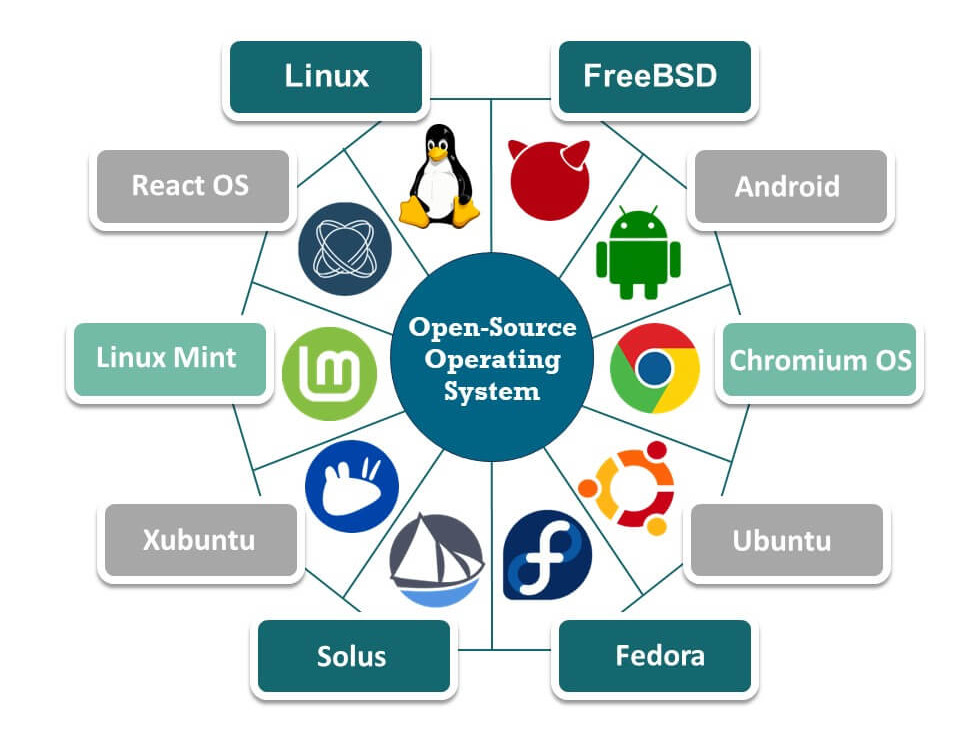
\includegraphics[scale=1.62]{Figures/0. General/sistemas_open_source.jpg}
  \caption{Tipos de sistemas \textit{open source}}
  \label{Tipos de sistemas open source}
\end{figure}

\newpage

\subsection{Sistemas operativos proprietários}

Enquanto os sistemas operativos de \textit{open source} promovem a colaboração, a transparência e a liberdade de personalização, os sistemas operativos proprietários oferecem conveniência, suporte profissional e uma experiência de utilizador refinada. \cite{advantagesOfProprietary}
\par \vspace{6pt}
A preferência por um tipo de sistema operativo sobre o outro muitas vezes reflete valores filosóficos, necessidades específicas de uso e considerações práticas, influenciando diretamente as decisões individuais e organizacionais de adoção de tecnologia.
\par \vspace{6pt}
Os sistemas operativos proprietários são desenvolvidos e mantidos por empresas que detêm os direitos de propriedade do software. As suas características são:

\begin{itemize}

  \item \textbf{Código Fechado}\\
  Os sistemas operativos proprietários são desenvolvidos por empresas que mantêm o código em segredo, limitando o acesso dos utilizadores à sua inspeção e modificação.
  
  \item \textbf{Controle Centralizado}\\
  As empresas que desenvolvem sistemas operativos proprietários exercem um controlo centralizado sobre o desenvolvimento, distribuição e suporte do software, o que pode limitar a flexibilidade e a capacidade de personalização pelos utilizadores.
  
  \item \textbf{Suporte Profissional}\\
  Os sistemas operativos proprietários geralmente são acompanhados por serviços de suporte profissional oferecidos pelas empresas, o que pode ser vantajoso para utilizadores e organizações que valorizam a garantia de suporte técnico especializado.
  
  \item \textbf{Restrições de Licença}\\
  Os sistemas operativos proprietários geralmente são distribuídos com licenças restritivas que limitam o uso, distribuição e modificação do software pelos utilizadores. 
  
  Essas restrições podem incluir proibições de redistribuição, limitações de uso em múltiplos dispositivos ou restrições de modificação do código-fonte.
  
  \item \textbf{Ciclos de Atualização Controlados}\\
  As atualizações de sistemas operativos proprietários são frequentemente controladas e fornecidas pelas empresas desenvolvedoras de acordo com um cronograma predeterminado. 
  
  Isso pode garantir uma maior consistência e estabilidade nas atualizações, mas também pode limitar a flexibilidade dos utilizadores em adotar novas funcionalidades ou correções de forma imediata.
\end{itemize}

\vspace{2pt}

\begin{figure}[H]
  \centering
  % width=\textwidth para imagem da largura do texto
  
\includegraphics[scale=0.2]{Figures/0. General/sistemas_proprietarios.jpg}
  \caption{Tipos de sistemas proprietários}
  \label{Tipos de sistemas proprietários}
\end{figure}
